\documentclass[11pt,letterpaper]{article}

%%%%%%%%%%%%%%%%%%%%%%%%%%%%%%%%% PAQUETES LIGEROS (COMPILACIÓN RÁPIDA) %%%%%%%%%%%%%%%%%%%%%%%%%%%%%%%%%
\usepackage[utf8]{inputenc}
\usepackage[T1]{fontenc}
\usepackage[spanish,es-tabla]{babel}
\usepackage{lmodern}
\usepackage{amsmath,amsfonts,amssymb}
\usepackage{graphicx}
\usepackage{float}
\usepackage[letterpaper,margin=2cm]{geometry}
\usepackage{booktabs,array}
\usepackage{enumitem}
\usepackage{titlesec}
\usepackage{parskip}
\usepackage{xcolor}
\usepackage[hidelinks]{hyperref}
\usepackage{url}
\usepackage{csquotes}
\graphicspath{{figuras/}{../figuras/}}

%%%%%%%%%%%%%%%%%%%%%%%%%%%%%%%%% ESTILO (formato tipo artículo) %%%%%%%%%%%%%%%%%%%%%%%%%%%%%%%%%
\renewcommand{\abstractname}{RESUMEN}
\titleformat{\section}{\Large\bfseries}{\thesection.}{0.6em}{}
\titleformat{\subsection}{\large\bfseries}{\thesubsection.}{0.6em}{}
\titlespacing*{\section}{0pt}{2.2ex plus 1ex minus .2ex}{1.5ex plus .2ex}

%%%%%%%%%%%%%%%%%%%%%%%%%%%%%%%%% MACROS %%%%%%%%%%%%%%%%%%%%%%%%%%%%%%%%%
\newcommand{\B}{\mathrm{B}}   % operador de rezago

%%%%%%%%%%%%%%%%%%%%%%%%%%%%%%%%% DOCUMENTO %%%%%%%%%%%%%%%%%%%%%%%%%%%%%%%%%
\begin{document}

%%%%%%%%%%%%%%%%%%%%%%%%%%%%%%%%% PORTADA %%%%%%%%%%%%%%%%%%%%%%%%%%%%%%%%%
\begin{center}
\IfFileExists{escudo.jpg}{\includegraphics[width=20mm]{escudo.jpg}\\[3mm]}{}
{\LARGE\bfseries \textbf{Tema:} Modelos ARIMA-X\\}
\vspace{4mm}
\begin{center}
    \Large \textbf{Modelación Dinámica de la Tasa de Intervención en Colombia: Un Enfoque ARIMAX con Efectos del Índice de Producción Industrial y Análisis de Intervención (2014-2026)}
\end{center}
\vspace{0.5cm}
{\large Seminario -- Grupo 3\par}
\vspace{4mm}
{\large \textbf{Integrantes:}\\ Walys Vera Herrera\\ Iván Andrés Durango Cogollo\\
Nicolás Buenaventura Schlesinger\par}
\vspace{1mm}
Universidad de Antioquia\\
Facultad de Ciencias Exactas y Naturales\\
Instituto de Matemáticas
\end{center}
\vspace{4mm}

% 2. RESUMEN / ABSTRACT
% ==========================================
\begin{abstract}
El presente trabajo aborda la modelación y el pronóstico dinámico de la Tasa de Intervención de Política Monetaria del Banco de la República de Colombia en función de la actividad del sector real, aproximada mediante el Índice de Producción Industrial (IPI), utilizando 152 observaciones mensuales comprendidas entre enero de 2014 y agosto de 2026. Ante la fuerte inercia temporal y la presencia de raíces unitarias en las series macroeconómicas, la regresión clásica por Mínimos Cuadrados Ordinarios colapsa estadísticamente al subestimar la varianza residual y generar inferencias espurias. Para solucionar esta deficiencia, se implementó la metodología ARIMAX (regresión con errores ARIMA) en conjunto con técnicas de análisis de intervención. 

Tras desestacionalizar el logaritmo del IPI mediante descomposición STL y confirmar un orden de integración $I(1)$ en ambas variables mediante pruebas ADF y KPSS, se utilizó el procedimiento de pre-blanqueamiento (\textit{prewhitening}) sobre la función de correlación cruzada (CCF), identificando que las variaciones en la producción industrial lideran las decisiones de política monetaria con retardos significativos de entre 3 y 6 meses. El modelo seleccionado mediante criterios de información (AIC y BIC) correspondió a una especificación con errores ARIMA$(4,1,1)$, complementada con una variable indicadora binaria (\textit{dummy}) que absorbió de manera efectiva el choque de varianza provocado por el confinamiento por COVID-19 (marzo a octubre de 2020). Las pruebas diagnósticas y la prueba de Ljung-Box sobre los residuos confirmaron el cumplimiento del supuesto de Ruido Blanco incorrelacionado ($p = 0.5876$). Finalmente, en la validación predictiva fuera de muestra (\textit{out-of-sample}) para los últimos 12 meses, se contrastó el desempeño de las especificaciones ARIMAX frente al modelo ARIMA univariado de referencia, evaluando el impacto de incorporar variables del sector real en la trayectoria pronosticada de la política monetaria a corto y mediano plazo.
\end{abstract}

\noindent\textbf{PALABRAS CLAVES:} Series de tiempo, ARIMA, ARIMA-X, variables exógenas, función de autocorrelación, pronóstico, Tasa de Intervención, Índice de Producción Industrial, Pre-blanqueamiento, Análisis de Intervención, Estacionariedad.

\section{Introducción}

Desde una perspectiva macroeconómica, la política monetaria de un país es un mecanismo dinámico que responde constantemente a las fluctuaciones de la economía real. En Colombia, el Banco de la República utiliza la Tasa de Intervención como su principal herramienta para controlar la inflación y estabilizar el ciclo económico. Por otro lado, el Índice de Producción Industrial (IPI), medido por el DANE, actúa como un termómetro directo de la actividad económica del país. Intuitivamente, existe una relación causal: los cambios en la producción industrial eventualmente motivan ajustes en las tasas de interés. 

Sin embargo, modelar esta relación estadísticamente presenta un desafío fundamental, pues si se intentara explicar la Tasa de Intervención ($Y_t$) en función del IPI ($X_t$) utilizando un modelo de regresión lineal clásico por Mínimos Cuadrados Ordinarios (MCO), se violaría el supuesto más crítico de la econometría: la independencia de los errores y como bien sabemos, las series de tiempo financieras y macroeconómicas poseen una fuerte inercia o ``memoria''; el valor de la tasa de interés de hoy está fuertemente condicionado por el valor de ayer, es por eso que ignorar esta dependencia temporal obliga al término de error del modelo a absorber dicha inercia, generando autocorrelación, subestimando la varianza real y produciendo inferencias estadísticas engañosas (falsos positivos).

Para abordar este problema de manera rigurosa, el presente trabajo adopta la metodología de los modelos ARIMAX (Regresión Dinámica con errores ARIMA). Este enfoque permite fusionar la capacidad explicativa de la econometría tradicional con la robustez estocástica de las series de tiempo. 

El objetivo general de este seminario es modelar y pronosticar la dinámica de la Tasa de Intervención del Banco de la República de Colombia en función del Índice de Producción Industrial, utilizando datos mensuales para el periodo 2014-2026. Para alcanzar esta meta, se plantean los siguientes objetivos específicos: diagnosticar el orden de integración de las series para evitar regresiones espurias, identificar los rezagos significativos mediante técnicas de pre-blanqueamiento, estimar los parámetros del modelo ARIMAX por Máxima Verosimilitud, y finalmente, evaluar la capacidad predictiva del modelo garantizando que los residuos finales se comporten como un ruido blanco puro.

%%%%%%%%%%%%%%%%%%%%%%%%%%%%%%%%%
\section{Marco teórico}
\subsection{Proceso Estocástico Débilmente Estacionario}
\label{sec:proceso_estocastico}
Un proceso estocástico $\{Y_t\}$ es débilmente estacionario si su función de medias $E[Y_t] = \mu_t = \mu$ y su función de varianza $\text{var}[Y_t] = \sigma_t^2 = \sigma^2$ son constantes e independientes del tiempo $t$, y además, la función de autocovarianza entre $Y_t$ y $Y_{t+h}$, dada por $\text{Cov}(Y_t, Y_{t+h}) = \gamma(h)$, depende únicamente del rezago $h$.

Dada la definición anterior, se dirá que:
\begin{itemize}
    \item Un proceso estocástico $\{Y_t\}$ es estacionario en media si su media es constante $\forall t$: $\mu_t = \mu$.
    \item Un proceso estocástico $\{Y_t\}$ es homogéneo si es estacionario en covarianza; es decir, su varianza es constante $\forall t$: $\sigma_t^2 = \sigma^2$.
\end{itemize}

\subsection{Serie de tiempo}
Una serie de tiempo puede definirse como una realización de un proceso estocástico $\{Y_t\}$; razón por la cual, se utilizará en repetidas ocasiones los términos definidos en la Sección \ref{sec:proceso_estocastico} para caracterizar una serie de tiempo.

\subsection{Modelos ARMA} 
Según Wei (2006, p. 57), en la construcción de modelos, frecuentemente, es necesario incluir términos autorregresivos y de media móvil de manera simultánea en un modelo. Este tipo de modelos son conocidos como Procesos Mixtos Autorregresivos de Medias Móviles $\text{ARMA}(p,q)$ y su especificación es la siguiente:

\begin{equation*}
\Phi(B)Y_t = \Theta(B)w_t
\end{equation*}

donde $p$ representa el orden del polinomio asociado a la componente autorregresiva $\Phi(B)$ y $q$ el orden del polinomio de la componente de media móvil $\Theta(B)$:
\begin{align*}
\Phi(B) &= 1 - \Phi_1 B - \Phi_2 B^2 - \dots - \Phi_p B^p \\
\Theta(B) &= 1 - \theta_1 B - \theta_2 B^2 - \dots - \theta_q B^q \quad \text{con} \quad w_t \sim RB(0, \sigma^2).
\end{align*}

Es importante mencionar que, si $\Phi(B)$ y $\Theta(B)$ no tienen raíces comunes (Wei, 2006, p. 57), el proceso puede caracterizarse como:

\begin{itemize}
    \item Estacionario si las raíces de $\Phi(B) = 0$ caen fuera del círculo unitario.
    \item Invertible si las raíces de $\Theta(B) = 0$ caen fuera del círculo unitario.
\end{itemize}


\subsection{Modelos ARIMA y necesidad de diferenciar} 
Según Wei (2006, p. 69), los procesos no estacionarios en media pueden presentar graves problemas a la hora de realizar la estimación sobre la media $\mu_t$ cuando no se conocen múltiples realizaciones del proceso. A pesar de ello, las series de tiempo homogéneas y no estacionarias en media pueden ser reducidas a series de tiempo estacionarias diferenciándolas cierta cantidad de veces (Wei, 2006, p. 71). Este tipo de modelos son conocidos como Procesos Autorregresivos Integrados de Media Móvil de orden $(p, d, q)$, denotados como $\text{ARIMA}(p, d, q)$ y su especificación es la siguiente: 

\[
\Phi(\B)(1-\B)^d\,Y_t=\Theta(\B)\,w_t ,
\]

donde $d$ representa el número de raíces unitarias del polinomio asociado a la componente autorregresiva, o equivalentemente, el número de veces que es necesario diferenciar para llegar a un proceso estacionario $\text{ARMA}(p,q)$.

\subsection{Modelos ARIMA-X}
Los modelos ARIMA-X son una extensión de los modelos ARIMA donde se introducen variables externas explicativas con el fin de conseguir una mejor predicción de la serie temporal (Ortiz Martín, 2022, p. 20). A estas variables externas explicativas se les conoce como variables exógenas.

Este modelo, de acuerdo con Amézquita Bravo (2021, p. 20), es utilizado, principalmente, para incorporar efectos de intervenciones o choques exógenos conocidos sobre cierta variable objetivo.

\subsubsection{Variable exógena}

Etimológicamente, la palabra \textit{exógena} proviene del griego: \textit{exo} (fuera). Una variable exógena es una variable observada $X_t$ cuyo valor viene determinado fuera del proceso que genera la serie $Y_t$ (DataCamp, 2024). Es decir, \textcolor{red!70!black}{el proceso que genera $Y_t$ no afecta el valor que tome $X_t$}, pero \textcolor{green!50!black}{sí puede ocurrir que $X_t$ afecte el valor que tome $Y_t$}.

Usualmente, una variable exógena se incorpora al modelo como regresora; es decir, puede ser utilizada como covariable para explicar el comportamiento de la serie $Y_t$. De acuerdo a Amézquita Bravo (2021, p. 20), las variables exógenas pueden entenderse como variables explicativas, \textit{dummies} o variables de intervención dentro del modelo de series de tiempo. Bajo la metodología ARIMA-X se asume que la serie observada está \textit{contaminada} por el efecto de variables de este tipo.

Para ilustrar esta distinción conceptual, supóngase que se desea analizar el rendimiento agrícola ($Y_t$) de un cultivo. Aunque la serie de tiempo puede estudiarse a partir de sus valores pasados, resulta conveniente incorporar la precipitación ($X_t$) para lograr un modelo más completo. En este escenario, es claro ver que \textcolor{green!50!black}{la cantidad de lluvia influye directamente sobre la cosecha}, por lo que $X_t$ actúa como variable explicativa para $Y_t$. Sin embargo, \textcolor{red!70!black}{la producción obtenida por el agricultor no altera la cantidad de precipitación}, lo que confirma que el efecto es estrictamente unidireccional y que $X_t$ puede considerarse una variable exógena que \textit{contamina} la serie de tiempo $\{Y_t\}$. 

Una representación de lo enunciado anteriormente puede detallarse en la Figura \ref{fig:relacion_exogena}.

\begin{figure}[H]
    \centering
    \IfFileExists{Ejemplo_Var_Exogena.png}{\includegraphics[width=0.75\textwidth]{Ejemplo_Var_Exogena.png}}{\fbox{Ejemplo\_Var\_Exogena.png}}
    \caption{Esquema de Precipitación como variable exógena del Rendimiento Agrícola}
    \label{fig:relacion_exogena}
\end{figure}

\subsubsection{Estructura específica del modelo ARIMA-X} 
\label{sec:espec_ARIMAX}
Suponga que conocemos $k$ variables exógenas $X_{1,t}, X_{2, t}, \dots, X_{k, t}$ que \textit{contaminan} cierta serie de tiempo $\{Y_t\}$ de la siguiente forma:
\begin{equation}
Y_t = \sum_{i=1}^k \beta_i X_{i,t} + \tilde{Y}_t
\label{eq:ARIMAX_1}
\end{equation}

donde $Y_t$ es la serie temporal observada, $X_{i,t}$ representa la $i$-ésima variable exógena a estudiar en el instante $t$, $\beta_i$ es el coeficiente que mide el impacto directo de la variable exógena $X_{i,t}$, y $\tilde{Y}_t$ corresponde a la denominada \textit{serie teórica}, la cual representa el comportamiento de la serie libre del efecto de las variables exógenas (Ortiz Martín, 2022, p. 20).

Despejando la serie teórica $\tilde{Y}_t$ de la Ecuación \ref{eq:ARIMAX_1} se obtiene la Ecuación \ref{eq:ARIMAX_2}:
\begin{equation}
\tilde{Y}_t = Y_t - \sum_{i=1}^k \beta_i X_{i,t}
\label{eq:ARIMAX_2}
\end{equation}

De este modo, la construcción de un modelo ARMA-X o ARIMA-X consiste en aplicar la metodología ARMA y ARIMA clásica sobre dicha serie teórica $\tilde{Y}_t$. 

Por ejemplo, según Ortiz Martín (2022, p. 20) un modelo $\text{ARMA-X}(p, q)$ no estacional adopta la siguiente forma:
\begin{equation}
\Phi(B) \left( Y_t - \sum_{i=1}^k \beta_i X_{i,t} \right) = \Theta(B) w_t
\label{eq:ARMAX_def}
\end{equation}

Y similarmente, la especificación de un Proceso Autorregresivo Integrado de Media Móvil de orden $(p, d, q)$ con variable exógena, denotado por $\text{ARIMA-X}(p,d,q)$, para la serie de tiempo $Y_t$ es dada por:
\begin{equation}
\Phi(B) (1-B)^d \left( Y_t - \sum_{i=1}^k \beta_i X_{i,t} \right) = \Theta(B) w_t
\label{eq:ARIMAX_def}
\end{equation}

donde $\Phi(B)$ y $\Theta(B)$ representan los operadores autorregresivo (AR) de orden $p$ y de media móvil (MA) de orden $q$ respectivamente, $d$ es el número de veces que hay que diferenciar para garantizar la estacionariedad y $w_t \sim RB(0, \sigma^2)$ denota el ruido blanco.


\subsubsection{Ejemplo de aplicación: Ajuste de ARIMA-X para pronosticar la demanda de transporte aéreo a corto y mediano plazo en Colombia} 
Para ilustrar una aplicación práctica de este modelo, Amézquita Bravo (2021) en su tesis de posgrado para optar el título de \textit{Magíster en Ciencias Económicas}, evalúa la demanda mensual de pasajeros en el transporte aéreo de Colombia ($Y_t$). En este estudio, el Producto Interno Bruto (PIB) actúa como la variable exógena explicativa ($X_{1,t}$), capturando el impacto positivo de la actividad económica sobre el volumen de pasajeros.

Siguiendo la Ecuación \ref{eq:ARIMAX_1}, el modelo ajustado se expresa como:
\begin{equation*}
Y_t = \beta_1 \text{PIB}_t + \tilde{Y}_t
\end{equation*}

donde el coeficiente $\beta_1$ cuantifica el efecto directo del PIB sobre la demanda de transporte aéreo. Al despejar la serie teórica $\tilde{Y}_t$ conforme a la Ecuación \ref{eq:ARIMAX_2}, se logra llegar a la estructura ARIMA tradicional explícita en la Ecuación \ref{eq:ARIMAX_def}:
\begin{equation*}
\Phi(B) (1-B)^d \tilde{Y}_t = \Theta(B) w_t \quad \implies \quad \Phi(B) (1-B)^d \left( Y_t - \beta_1 \text{PIB}_t \right) = \Theta(B) w_t
\end{equation*}

Cabe destacar que en la investigación también se evaluaron otras variables candidatas, como el precio del petróleo y choques exógenos locales e internacionales; sin embargo, su efecto resultó no significativo (Amézquita Bravo, 2021). 

De acuerdo con el resumen del trabajo de Amézquita Bravo (2021), la inclusión del PIB como variable exógena en la estructura ARIMA-X mejoró la precisión del modelo, reduciendo los errores de pronóstico (MAPE y RMSE) por debajo del umbral del 3\% (Amézquita Bravo, 2021); lo que, de alguna u otra manera, nos habla sobre la utilidad de estos modelos.

\subsubsection{Estructura del Modelo ARIMA-X propuesta por Fan (2009)}
\label{sec:gen_ARIMAX}

La estructura presentada en la Ecuación \ref{eq:ARIMAX_1} asume una relación estática e instantánea entre las covariables y la respuesta. Sin embargo, cuando se consideran $k$ variables exógenas $X_{1,t}, X_{2,t}, \dots, X_{k,t}$, es común que cada una afecte a la serie $Y_t$ a través de sus rezagos. Para capturar este comportamiento dinámico, Fan (2009, p. 157) propone la siguiente estructura general:

\begin{equation}
Y_t = \sum_{i=1}^k v_i(B) X_{i,t} + \underbrace{\frac{\Theta(B)}{\Phi(B)(1-B)^d} w_t}_{\tilde{Y}_t} = \sum_{i=1}^k v_i(B) X_{i,t} + \tilde{Y}_t
\label{eq:ARIMAX_general}
\end{equation}

donde, manteniendo la notación unificada para el sistema, cada componente se interpreta de la siguiente manera (Fan, 2009, p. 157):
\begin{itemize}
    \item $k$: Número total de variables exógenas consideradas en el sistema.
    \item $v_i(B) = v_{i,0} + v_{i,1}B + v_{i,2}B^2 + \dots$: Polinomio de retardos que expresa el efecto dinámico de la $i$-ésima variable exógena como una combinación lineal de sus propios rezagos:
    \[
    v_i(B)X_{i,t} = \sum_{j=0}^{\infty} v_{i,j} X_{i,t-j} = v_{i,0}X_{i,t}+v_{i,1}X_{i,t-1}+v_{i,2}X_{i,t-2}+ \dots
    \]
    \item $\tilde{Y}_t$: Serie de tiempo teórica libre del efecto de las variables exógenas, modelada mediante la estructura ARIMA habitual con $w_t \sim \text{RB}(0, \sigma^2)$.
\end{itemize}

\vspace{0.3cm}

\textbf{Observación:}
Para deducir la Ecuación \ref{eq:ARIMAX_1} a partir de la formulación general (Ecuación \ref{eq:ARIMAX_general}), se aplican dos supuestos sobre el comportamiento del sistema:
\begin{enumerate}
\item El impacto contemporáneo de la variable exógena $X_t$ se asume constante sobre $Y_t$, definiendo $v_{i,0} = \beta_i$.
\item Los rezagos de la variable exógena $X_{t-1}, X_{t-2}, \dots$ no generan efectos sobre $Y_t$, por lo que $v_{i,j} = 0$ $\forall j \geq 1$.
\end{enumerate}

Bajo estas condiciones, el polinomio de retardos $v_i(B)$ se vuelve un escalar constante:
\begin{equation*}
v_i(B) = \beta_i + 0 \cdot B + 0 \cdot B^2 + \dots = \beta_i
\end{equation*}

Y finalmente, sustituyendo $v_i(B) = \beta_i$ directamente en la Ecuación \ref{eq:ARIMAX_general}, se obtiene la expresión:
\[Y_t = \sum_{i=1}^k \beta_i X_{i,t} + \tilde{Y}_t\] 
demostrando así que lo mencionado en la Sección \ref{sec:espec_ARIMAX} es un caso específico de la estructura propuesta en esta Sección.

Asimismo, para identificar en la práctica cuáles rezagos del polinomio $v_i(B)$ son significativos sin que la autocorrelación interna de cada serie distorsione el análisis, Fan (2009, p. 157, sec. 4) establece el procedimiento de filtrado o pre-blanqueamiento (\textit{prewhitening}): primero se ajusta un modelo ARMA a la $i$-ésima serie de entrada estacionaria (en diferencias, $\nabla X_{i,t}$) tal que $\Phi_i(B)\nabla X_{i,t} = \Theta_i(B)\alpha_{i,t}$, de donde se despeja la innovación de ruido blanco:
\begin{equation}
\alpha_{i,t} = \frac{\Phi_i(B)}{\Theta_i(B)}\nabla X_{i,t} \sim \text{RB}(0, \sigma_\alpha^2).
\label{eq:fan_alfa}
\end{equation}
Posteriormente, se filtra la serie de salida estacionaria $\nabla Y_t$ utilizando exactamente los mismos polinomios de entrada $\Phi_i(B)$ y $\Theta_i(B)$ para obtener:
\begin{equation}
\beta_{i,t} = \frac{\Phi_i(B)}{\Theta_i(B)}\nabla Y_t ,
\label{eq:fan_beta}
\end{equation}
y se calcula la función de correlación cruzada (CCF) entre $\alpha_{i,t}$ y $\beta_{i,t}$ para identificar el grado de retardo con el que $X_{i,t}$ impacta a $Y_t$ (Fan, 2009, p. 157; Shumway y Stoffer, 2017).

\subsubsection{Análisis de intervención}
Es la parte de la metodología que permite decidir si una acción o fenómeno concreto ha tenido repercusión en la evolución de la serie, es decir, si cambió su estructura (Ortiz Martín, 2022, sec.~3.5.3; Peña, 2005). Su objetivo no es pronosticar sino hacer inferencia sobre si la intervención tiene un efecto significativo (Ortiz Martín, 2022, sec.~3.5.3). Siguiendo a Box y Tiao (1975), el modelo es
\[
Y_t=\frac{\omega(\B)}{\delta(\B)}\,\xi_t+\tilde{Y}_t ,
\]
donde $\tilde{Y}_t$ es un ruido ARIMA y $\xi_t$ es una variable indicadora de la intervención en la fecha $T$: un \emph{pulso}, $P_t=\mathbf{1}_{\{t=T\}}$, para un evento puntual, o un \emph{escalón}, $S_t=\mathbf{1}_{\{t\ge T\}}$, para un cambio que se mantiene. En el caso más simple, $Y_t=\omega\,S_t+\tilde{Y}_t$, y el efecto es un cambio de nivel de tamaño $\omega$. Se contrasta $H_0$: la intervención no afecta a la serie, frente a $H_1$: sí la afecta (Ortiz Martín, 2022, sec.~3.5.3), lo que equivale a evaluar si $\omega$ es significativamente distinto de cero.

\subsubsection{Valores atípicos}
Cuando un hecho exógeno cambia la dinámica natural de la serie, aparecen atípicos que pueden verse como variables externas de existencia no previsible; es decir, son intervenciones cuya fecha y tipo se desconocen y deben detectarse a partir de los datos (Ortiz Martín, 2022, sec.~3.5.4). Con $T_0$ el momento del evento, se consideran tres tipos, cuyas funciones de transferencia son (Ortiz Martín, 2022, sec.~3.5.4):
\begin{itemize}[nosep]
\item \emph{Atípico aditivo (AO):} afecta solo un instante, $X_t=\mathbf{1}_{\{t=T_0\}}$.
\item \emph{Cambio transitorio (TC):} el efecto decae de forma exponencial, $X_t=\delta^{\,t-T_0}\mathbf{1}_{\{t\ge T_0\}}$, usualmente con $\delta=0.7$.
\item \emph{Cambio de nivel (LS):} el efecto se mantiene, $X_t=\mathbf{1}_{\{t\ge T_0\}}$.
\end{itemize}
Chen y Liu (1993) proponen un procedimiento iterativo que detecta los atípicos y estima de forma conjunta los parámetros del modelo y los efectos de los atípicos mediante regresión múltiple; además de los tres tipos anteriores, distinguen el atípico innovacional (IO). El tratamiento consiste en identificar el momento y el tipo del atípico, medir su impacto, reconstruir la serie sin el efecto del evento y aplicar la metodología de Box--Jenkins a la serie resultante; con un atípico de tipo LS hay que ajustar también las predicciones (Ortiz Martín, 2022, sec.~3.5.4).


\subsubsection{Identificación, estimación, diagnóstico y pronóstico}
La implementación completa del modelo sigue el ciclo iterativo de Box y Jenkins (Shumway y Stoffer, 2017):
\begin{enumerate}
    \item \textbf{Identificación y estacionariedad:} Se determina el orden de integración $d$ mediante pruebas formales de raíz unitaria como la prueba de Dickey-Fuller Aumentada (ADF) (Dickey y Fuller, 1979) y la prueba estacionaria de Kwiatkowski-Phillips-Schmidt-Shin (KPSS) (Kwiatkowski et al., 1992), examinando posteriormente la ACF y PACF de la serie diferenciada.
    \item \textbf{Estimación y selección:} Los parámetros $\boldsymbol{\beta}$, $\boldsymbol{\phi}$, $\boldsymbol{\theta}$ y $\sigma_w^2$ se estiman conjuntamente maximizando la función de log-verosimilitud exacta (vía representación en espacio de estados y filtro de Kalman), seleccionando la especificación que minimiza los criterios de información de Akaike ($\text{AIC} = -2\ln(\hat{L}) + 2K$) y Bayesiano de Schwarz ($\text{BIC} = -2\ln(\hat{L}) + K\ln(T_{\text{eff}})$) (Ortiz Martín, 2022, sec.~3.4).
    \item \textbf{Diagnóstico de residuos:} Los residuos estandarizados $\hat{w}_t$ deben comportarse como un Ruido Blanco. Para contrastar la hipótesis nula conjunta de ausencia de autocorrelación hasta el rezago $H$ ($H_0: \rho_w(1) = \dots = \rho_w(H) = 0$) se emplea el estadístico de Ljung y Box (1978):
    \begin{equation}
    Q(H) = T_{\text{eff}}(T_{\text{eff}}+2)\sum_{h=1}^{H} \frac{\hat{\rho}_{\hat{w}}^2(h)}{T_{\text{eff}}-h} \underset{H_0}{\overset{a}{\sim}} \chi^2_{H - p - q} ,
    \label{eq:ljung_box}
    \end{equation}
    donde los grados de libertad se corrigen restando exclusivamente el número de parámetros autorregresivos y de medias móviles estimados ($p + q$) (Hyndman y Athanasopoulos, 2021).
    \item \textbf{Pronóstico:} Para proyectar $Y_{T+h}$ con un modelo ARIMA-X es indispensable disponer de los valores futuros de las regresoras exógenas $X_{T+h}$, ya sea mediante evaluación \textit{ex-post} (utilizando los valores observados en un conjunto de validación reservado) o mediante proyección \textit{ex-ante} (pronosticando previamente las covariables o definiendo escenarios macroeconómicos) (Hyndman y Athanasopoulos, 2021).
\end{enumerate}


% \subsubsection{Identificación, diagnóstico y predicción}
% La construcción del modelo sigue las etapas de Box--Jenkins: identificación de los órdenes con la función de autocorrelación (ACF) y de autocorrelación parcial (PACF) (Shumway y Stoffer, 2017), estimación, validación de los residuos con la prueba de Ljung--Box (Ljung y Box, 1978) y selección del modelo con criterios de información como AIC y BIC (Ortiz Martín, 2022, sec.~3.4). Para pronosticar con un modelo ARIMA-X se necesitan los valores futuros de las regresoras: los de calendario se conocen, y los demás deben pronosticarse o fijarse mediante escenarios (Hyndman y Athanasopoulos, 2021).

%%%%%%%%%%%%%%%%%%%%%%%%%%%%%%%%%
% 6. OBJETIVOS
% ==========================================
\section{Objetivos}

\subsection{Objetivo General}
Modelar y evaluar la dinámica temporal de la Tasa de Intervención de Política Monetaria del Banco de la República de Colombia en función del Índice de Producción Industrial (IPI) durante el periodo 2014-2026, utilizando la metodología de regresión dinámica con errores ARIMA (ARIMAX).

\subsection{Objetivos Específicos}
\begin{itemize}
    \item Diagnosticar el orden de integración de las series macroeconómicas mediante pruebas formales de raíz unitaria para evitar el riesgo de regresión espuria.
    \item Identificar la estructura de rezagos causales entre el IPI y la Tasa de Intervención aplicando técnicas de pre-blanqueamiento (\textit{prewhitening}) y análisis de correlación cruzada (CCF).
    \item Incorporar el análisis de intervención mediante variables indicadoras (\textit{dummies}) para aislar y cuantificar el choque estructural provocado por la pandemia de COVID-19 en la varianza del modelo.
    \item Estimar los parámetros del modelo ARIMAX por Máxima Verosimilitud y validar los supuestos estocásticos de los residuos (Ruido Blanco y Normalidad).
    \item Evaluar el desempeño predictivo del modelo ajustado mediante un ejercicio de pronóstico fuera de muestra (\textit{out-of-sample}), utilizando métricas de error estándar.
\end{itemize}


%%%%%%%%%%%%%%%%%%%%%%%%%%%%%%%%%
% 7. METODOLOGÍA
% ==========================================
\section{Metodología}

El presente trabajo adopta un enfoque cuantitativo, empírico y analítico basado en la metodología de Box y Jenkins para el modelado de series de tiempo univariadas y su extensión a modelos de regresión dinámica con variables exógenas (ARIMAX) expuesta en el Marco Teórico. Todos los procedimientos computacionales, transformaciones, pruebas de hipótesis, estimaciones y diagnósticos se desarrollaron en el entorno estadístico \texttt{R}.

La estrategia metodológica se estructuró de forma rigurosa en seis etapas secuenciales:

\begin{enumerate}
    \item \textbf{Consolidación y Tratamiento Preliminar de Datos:}
    Se utilizó una muestra mensual de 152 observaciones continuas comprendidas entre enero de 2014 y agosto de 2026 ($T = 152$). 
    \begin{itemize}
        \item \textit{Variable objetivo ($Y_t$):} Tasa de Intervención de Política Monetaria del Banco de la República. Dado que la fuente original registra datos diarios, se convirtieron a frecuencia mensual calculando el promedio aritmético de cada mes, imputando días no hábiles mediante el método de arrastre de la última observación observada (\textit{LOCF: Last Observation Carried Forward}).
        \item \textit{Variable exógena ($X_t$):} Índice de Producción Industrial (IPI), publicado por el DANE. Para corregir la no linealidad y el marcado patrón estacional anual identificado en la serie, se aplicó la transformación logarítmica y posteriormente una desestacionalización robusta mediante descomposición STL (\textit{Seasonal and Trend decomposition using Loess}) con ventana periódica. La serie final desestacionalizada ($X_t$) se escaló como $100 \times \ln(\text{IPI}_{SA})$, de modo que una variación unitaria represente aproximadamente un cambio del $1\%$ en la producción industrial real.
    \end{itemize}

    \item \textbf{Diagnóstico de Estacionariedad en Media (Raíces Unitarias):}
    Con el fin de evitar estimaciones espurias y determinar el orden de integración $d$ requerido en las Ecuaciones \ref{eq:ARIMAX_def} y \ref{eq:ARIMAX_general}, se evaluó la estacionariedad de $Y_t$ y $X_t$ a través de dos pruebas estadísticas complementarias:
    \begin{itemize}
        \item La prueba de Dickey-Fuller Aumentada (ADF), con hipótesis nula de existencia de raíz unitaria ($H_0: \text{la serie no es estacionaria}$).
        \item La prueba de Kwiatkowski-Phillips-Schmidt-Shin (KPSS), con hipótesis nula de estacionariedad ($H_0: \text{la serie es estacionaria}$).
    \end{itemize}
    Se aplicó el operador de primera diferencia ordinaria $\nabla = (1 - B)$ sobre ambas series para garantizar la condición de estacionariedad débil ($d=1$).

    \item \textbf{Pre-blanqueamiento y Selección de Rezagos Exógenos (CCF):}
    Dado que una regresión directa entre series autocorrelacionadas induce correlaciones cruzadas artificiales, se ejecutó el procedimiento de pre-blanqueamiento (\textit{prewhitening}) siguiendo exactamente los pasos definidos por Fan (2009, p. 157) en las Ecuaciones \ref{eq:fan_alfa} y \ref{eq:fan_beta}:
    \begin{enumerate}
        \item[a.] Se ajustó un modelo ARIMA univariado óptimo a la variable exógena diferenciada $\nabla X_t = (1-B)X_t$ para extraer sus innovaciones puras mediante los polinomios autorregresivo $\Phi_X(B)$ y de media móvil $\Theta_X(B)$:
        \[
        \alpha_t = \frac{\Phi_X(B)}{\Theta_X(B)} \nabla X_t, \quad \text{garantizando que } \alpha_t \sim RB(0, \sigma_\alpha^2).
        \]
        \item[b.] Se filtró la serie objetivo diferenciada $\nabla Y_t = (1-B)Y_t$ con exactamente los mismos polinomios estimados para el IPI:
        \[
        \beta_t = \frac{\Phi_X(B)}{\Theta_X(B)} \nabla Y_t.
        \]
        \item[c.] Se calculó la Función de Correlación Cruzada (CCF) entre las series pre-blanqueadas $\text{CCF}(\alpha_{t+k}, \beta_t)$. Aquellos rezagos negativos ($k < 0$) cuyos coeficientes superaron las bandas de confianza de Bartlett al $95\%$ ($\pm 1.96/\sqrt{T}$) se seleccionaron como retardos causales significativos (3 y 6 meses) para incorporarse en el polinomio $v_1(B)$ de la Ecuación \ref{eq:ARIMAX_general}.
    \end{enumerate}

    \item \textbf{Diseño de Intervención Estructural (Dummy Pandemia):}
    Para aislar la anomalía observada en el periodo 2020 debida a la emergencia sanitaria por COVID-19, se construyó una variable de intervención de tipo pulso extendido:
    \begin{equation}
        D_{t}^{\text{COVID}} = \begin{cases} 
        1, & \text{si marzo de 2020} \le t \le \text{octubre de 2020} \\ 
        0, & \text{en cualquier otro caso} 
        \end{cases}
        \label{eq:dummy_covid}
    \end{equation}
    Esta variable se incluyó en la matriz exógena para proteger la estimación frente a quiebres estructurales severos.

    \item \textbf{Estimación y Comparación de Modelos Competitivos:}
    Una vez recortados los primeros 6 meses consumidos por el rezago de orden 6 ($X_{t-6}$), la muestra efectiva común de 146 observaciones (julio 2014 a agosto 2026) se dividió en un conjunto de entrenamiento de 134 meses (julio 2014 a agosto 2025) y una ventana de validación fuera de muestra (\textit{out-of-sample}) de $h = 12$ meses (septiembre 2025 a agosto 2026). Sobre el conjunto de entrenamiento se ajustaron por Máxima Verosimilitud tres especificaciones:
    \begin{itemize}
        \item \textbf{Modelo 0 (Benchmark univariado):} $\text{ARIMA}(p,d,q)$ puro sobre la tasa de intervención $Y_t$.
        \item \textbf{Modelo 1 (ARIMAX contemporáneo):} Caso específico definido en la Ecuación \ref{eq:ARIMAX_def}, incorporando el IPI desestacionalizado contemporáneo ($X_{1,t}$) y la variable Dummy de COVID-19 ($D_t^{\text{COVID}}$).
        \item \textbf{Modelo 2 (ARIMAX con rezagos):} Estructura dinámica general de Fan (2009) definida en la Ecuación \ref{eq:ARIMAX_general}, incorporando el polinomio de retardos del IPI $v_1(B)X_{1,t} = v_{1,0}X_{1,t} + v_{1,3}X_{1,t-3} + v_{1,6}X_{1,t-6}$ junto con la Dummy de COVID-19.
    \end{itemize}
    La selección de los órdenes autorregresivos $p$ y de medias móviles $q$ se realizó minimizando los criterios de información de Akaike (AIC) y Bayesiano de Schwarz (BIC).

    \item \textbf{Diagnóstico Residual y Validación Predictiva:}
    Para validar que los residuos estimados $\hat{w}_t$ satisfagan el supuesto de Ruido Blanco, se aplicó la prueba de Ljung-Box sobre 24 rezagos, ajustando los grados de libertad por los parámetros ARMA estimados ($\text{df} = 24 - p - q$), además de la prueba de normalidad de Shapiro-Wilk. Finalmente, se generaron los pronósticos para los 12 meses del horizonte de prueba y se evaluó el desempeño predictivo mediante tres métricas de error: la Raíz del Error Cuadrático Medio (RMSE), el Error Absoluto Medio (MAE) y el Error Porcentual Absoluto Medio (MAPE).
\end{enumerate}


%%%%%%%%%%%%%%%%%%%%%%%%%%%%%%%%%
% 8. APLICACIÓN
% ==========================================
\section{Aplicación}

En esta sección se presentan los resultados de aplicar la metodología ARIMAX a los datos macroeconómicos colombianos. El procesamiento, estimación y validación se realizaron utilizando el software estadístico \texttt{R}.

\subsection{Descripción de los Datos y Análisis Exploratorio}
El conjunto de datos comprende observaciones de frecuencia mensual desde enero de 2014 hasta agosto de 2026 ($T = 152$ observaciones). La variable objetivo de interés es la Tasa de Intervención de Política Monetaria del Banco de la República ($Y_t$), mientras que la variable exógena es el Índice de Producción Industrial (IPI) calculado por el DANE. La Tabla \ref{tab:descriptivas} presenta el resumen descriptivo arrojado por el procesamiento de los datos: en abril de 2020 el IPI registró una caída del $-30.8\%$ frente a febrero de 2020 (alcanzando su mínimo de $69.03$), mientras que la tasa de intervención fluctuó entre un mínimo de $1.75\%$ en octubre de 2020 y un máximo de $13.25\%$ en junio de 2023.

\begin{table}[H]
\centering
\caption{Resumen descriptivo de las series originales y transformadas (2014:01 -- 2026:08, $T = 152$).}
\label{tab:descriptivas}
\vspace{2mm}
\begin{tabular}{lcccccc}
\toprule
\textbf{Variable} & \textbf{Media} & \textbf{Desv. Est.} & \textbf{Mínimo} & \textbf{Máximo} & \textbf{Fecha Mín.} & \textbf{Fecha Máx.} \\
\midrule
IPI original ($\text{IPI}_t$) & $101.20$ & $6.45$ & $69.03$ & $114.72$ & 2020-04-01 & 2022-11-01 \\
Tasa de Intervención ($Y_t$, \%) & $6.58$ & $3.51$ & $1.75$ & $13.25$ & 2020-10-01 & 2023-06-01 \\
IPI desestacionalizado ($X_t = 100\ln(\text{IPI}_{SA})$) & $461.55$ & $5.97$ & $426.64$ & $471.57$ & 2020-04-01 & 2023-03-01 \\
\bottomrule
\end{tabular}
\end{table}

\begin{figure}[H]
    \centering
    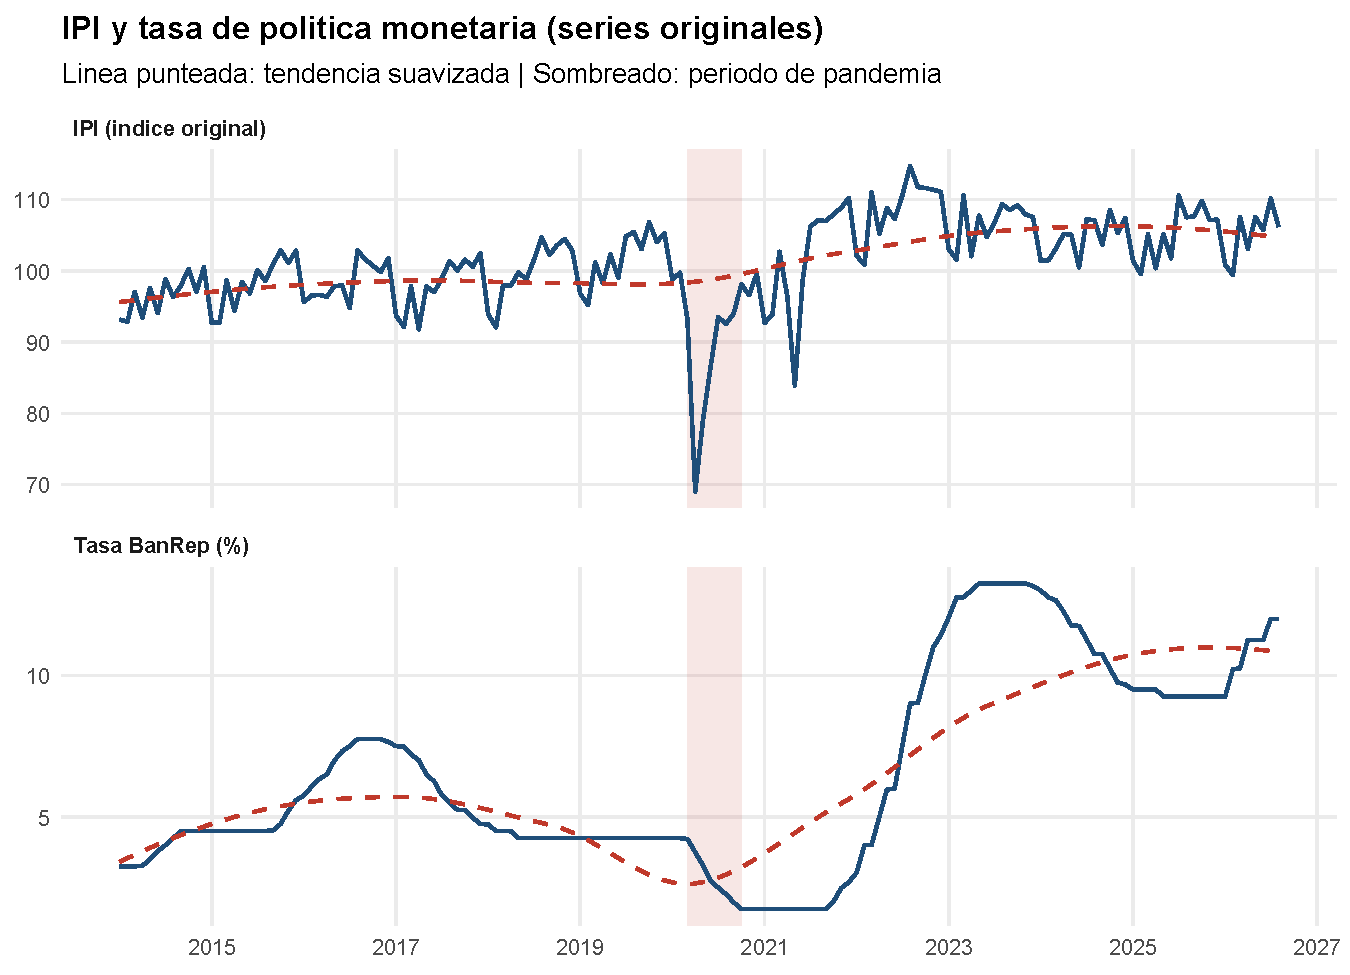
\includegraphics[width=0.95\textwidth]{01_series_originales.pdf}
    \caption{Evolución histórica del IPI y la Tasa de Intervención (2014-2026).}
    \label{fig:series_originales}
\end{figure}

Como se observa en la Figura \ref{fig:series_originales}, ambas series exhiben un comportamiento no estacionario en media, caracterizado por tendencias estocásticas cambiantes. Es particularmente notable el choque estructural exógeno ocurrido en el primer semestre de 2020 (franja sombreada), correspondiente a las medidas de confinamiento por la pandemia de COVID-19. Este evento provocó una caída sin precedentes en la producción industrial, seguida de una reducción drástica en la tasa de intervención como medida de política monetaria expansiva.

Adicionalmente, el IPI presenta un fuerte componente estacional determinístico. Al analizar el gráfico estacional (Figura \ref{fig:estacionalidad}), se evidencia un patrón repetitivo anual, con caídas sistemáticas en meses específicos (como abril, asociado a la Semana Santa). Para evitar que esta estacionalidad contamine la relación causal con la tasa de interés (la cual no es estacional, con $D=0$ según la prueba OCSB), se procedió a desestacionalizar el logaritmo del IPI utilizando el método de descomposición STL, obteniendo la serie ajustada $X_t$ que se utiliza como regresora.

\begin{figure}[H]
    \centering
    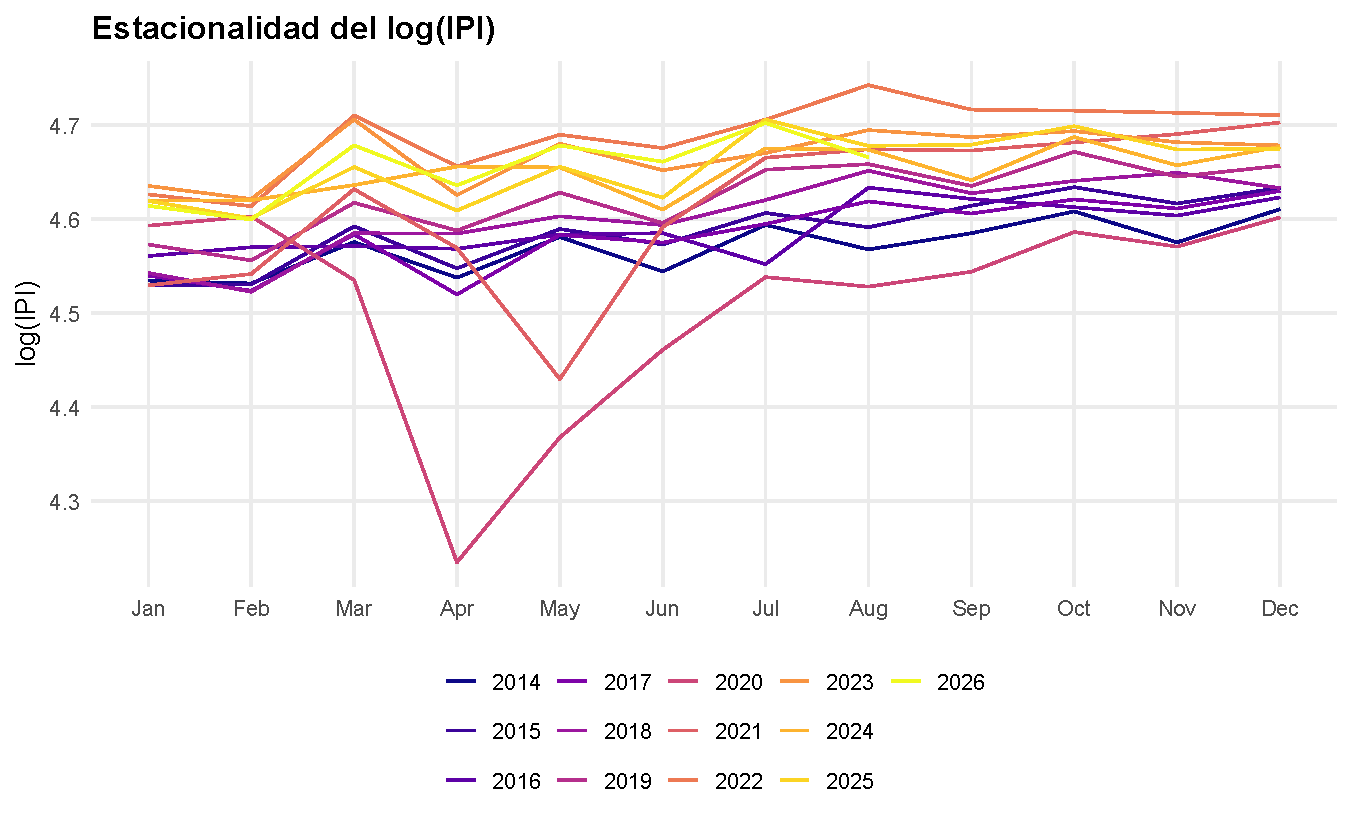
\includegraphics[width=0.85\textwidth]{02_estacionalidad.pdf}
    \caption{Gráfico estacional del logaritmo del IPI.}
    \label{fig:estacionalidad}
\end{figure}

\subsection{Análisis de Estacionariedad}
Para evitar el fenómeno de regresión espuria, es imperativo garantizar que las series modeladas sean estacionarias. La Tabla \ref{tab:estacionariedad} presenta los $p$-valores arrojados por las pruebas formales de Dickey-Fuller Aumentada (ADF) y KPSS en niveles y en primera diferencia. Los resultados confirmaron la presencia de una raíz unitaria en los niveles de ambas series ($p\text{-valor KPSS} = 0.0100 < 0.05$). Por consiguiente, se aplicó el operador de primera diferencia $\nabla = (1-B)$ tanto a la Tasa de Intervención como al IPI desestacionalizado ($d = 1$), tras lo cual la prueba KPSS confirmó estacionariedad en media ($p\text{-valor} = 0.1000 > 0.05$) en ambas variables diferenciadas.

\begin{table}[H]
\centering
\caption{Resultados de las pruebas de estacionariedad ADF y KPSS en niveles y primera diferencia ($d=1$).}
\label{tab:estacionariedad}
\vspace{2mm}
\begin{tabular}{lccc}
\toprule
\textbf{Serie} & \textbf{ADF ($p$-valor)} & \textbf{KPSS ($p$-valor)} & \textbf{Decisión ($d$)} \\
\midrule
Tasa ($Y_t$) & $0.1818$ & $0.0100$ & No estacionaria ($d=1$) \\
$\nabla$ Tasa ($\nabla Y_t$) & $0.3568^*$ & $0.1000$ & Estacionaria por KPSS \\
IPI desest. ($X_t$) & $0.1292$ & $0.0100$ & No estacionaria ($d=1$) \\
$\nabla$ IPI desest. ($\nabla X_t$) & $0.0100$ & $0.1000$ & Estacionaria ($I(0)$) \\
\bottomrule
\multicolumn{4}{l}{\footnotesize $^*$Nota: En $\nabla Y_t$, la alta persistencia autorregresiva reduce la potencia del test ADF con rezagos fijos,} \\
\multicolumn{4}{l}{\footnotesize pero el test KPSS ($p \ge 0.10$) y la selección por `ndiffs` confirman que una diferencia ($d=1$) es suficiente.}
\end{tabular}
\end{table}

\begin{figure}[H]
    \centering
    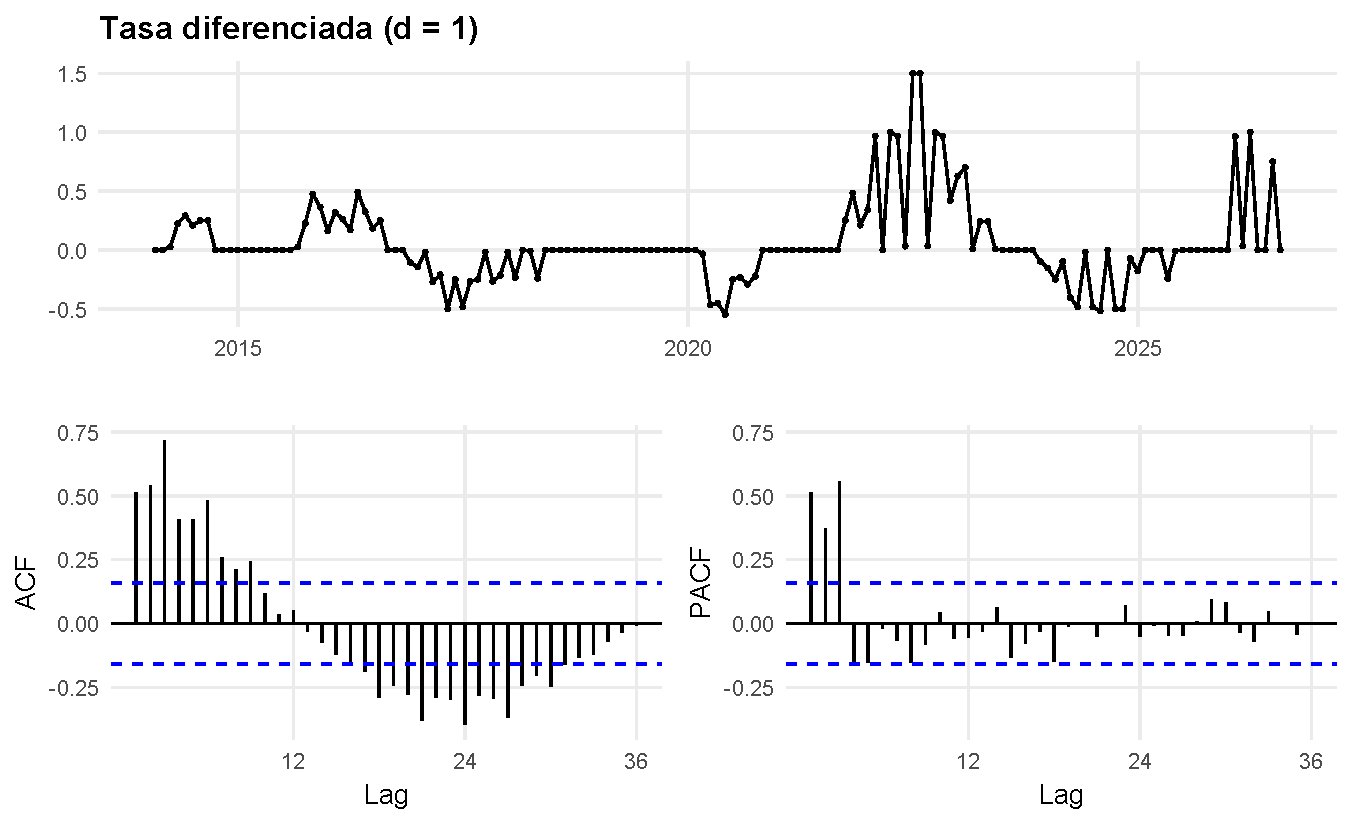
\includegraphics[width=0.9\textwidth]{03_acf_pacf.pdf}
    \caption{Tasa de Intervención diferenciada ($d=1$) con sus respectivas funciones ACF y PACF.}
    \label{fig:tasa_diff}
\end{figure}

La Figura \ref{fig:tasa_diff} muestra la serie diferenciada ($\nabla Y_t$), la cual ahora oscila alrededor de una media constante de cero, cumpliendo el primer momento de la estacionariedad. Las funciones de Autocorrelación (ACF) y Autocorrelación Parcial (PACF) de esta serie diferenciada revelan una estructura de dependencia temporal significativa en los primeros cuatro rezagos, justificando la necesidad de un componente ARMA para modelar la serie teórica $\tilde{Y}_t$.

\subsection{Identificación Estructural (Pre-blanqueamiento)}
Para determinar la estructura de rezagos con la que la producción industrial afecta la política monetaria conforme a las Ecuaciones \ref{eq:fan_alfa} y \ref{eq:fan_beta}, se aplicó la técnica de pre-blanqueamiento. Se ajustó un modelo ARIMA univariado al IPI desestacionalizado ($\text{ARIMA}(0,1,2)$) y se filtró la Tasa de Intervención con los mismos coeficientes, eliminando así la autocorrelación interna de las series.

\begin{figure}[H]
    \centering
    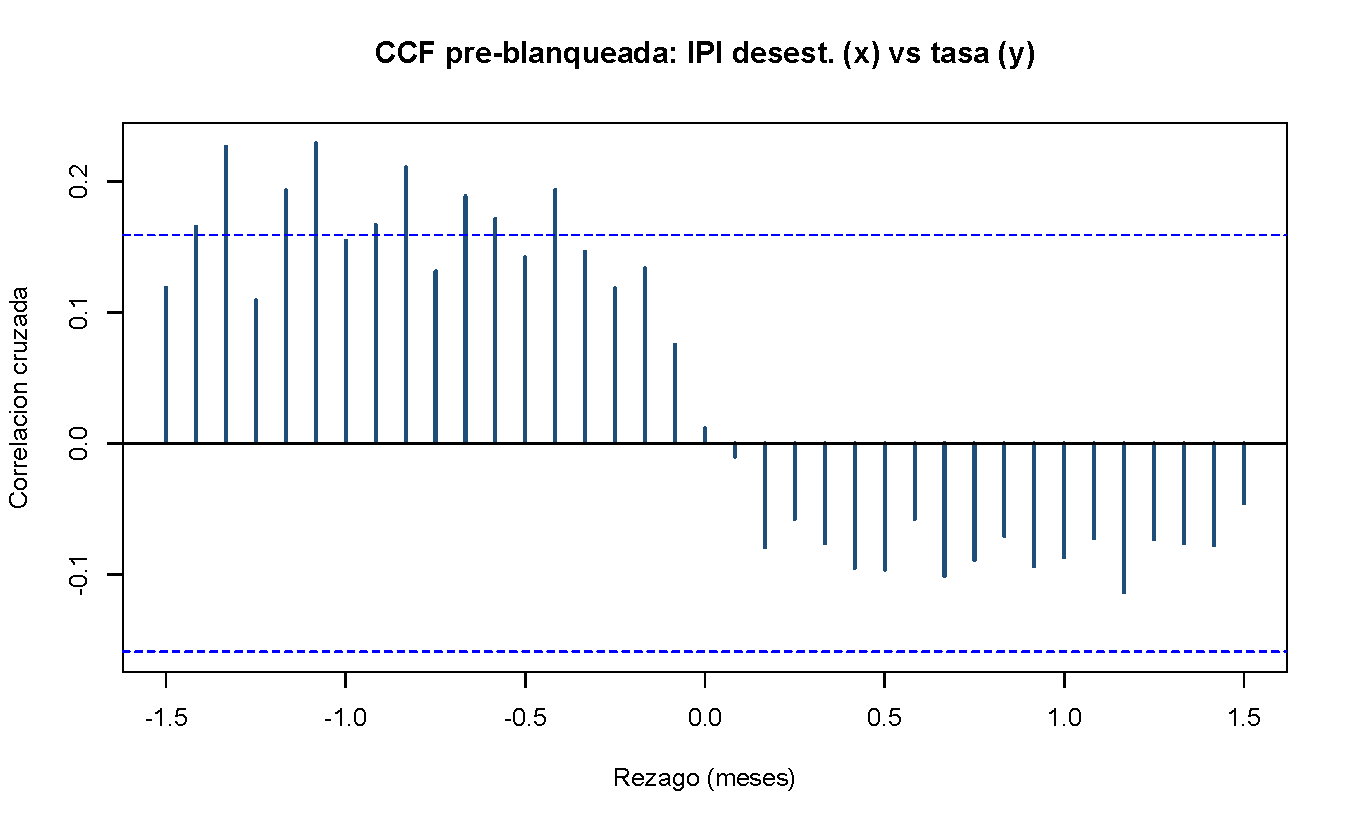
\includegraphics[width=0.8\textwidth]{04_ccf.pdf}
    \caption{Función de Correlación Cruzada (CCF) pre-blanqueada entre el IPI y la Tasa.}
    \label{fig:ccf}
\end{figure}

La Figura \ref{fig:ccf} presenta la CCF resultante. Es fundamental notar que en \texttt{R}, para series mensuales de frecuencia 12, el eje de rezagos se imprime en fracciones de año (donde $-0.25$ equivale al mes $-3$ y $-0.50$ al mes $-6$). Se observan correlaciones cruzadas significativas exclusivamente en el lado izquierdo del gráfico (rezagos negativos), lo que indica estadísticamente que las innovaciones en el IPI ($X_t$) anteceden y lideran los cambios en la Tasa de Intervención ($Y_t$) entre 3 y 6 meses, sin evidencia de retroalimentación en los rezagos positivos. Basado en esta evidencia empírica, se justifica la inclusión de los rezagos 3 y 6 del IPI en la Ecuación \ref{eq:ARIMAX_general}.

\subsection{Estimación y Diagnóstico del Modelo ARIMAX}
Siguiendo las especificaciones del Marco Teórico, se estimaron el Modelo 1 (estructura contemporánea de la Ecuación \ref{eq:ARIMAX_def}) y el Modelo 2 (estructura con rezagos de la Ecuación \ref{eq:ARIMAX_general}). Minimizando el Criterio de Información de Akaike (AIC), el algoritmo seleccionó una estructura de errores \textbf{ARIMA(4,1,1)}. La Tabla \ref{tab:coeficientes} presenta los coeficientes estimados por Máxima Verosimilitud para ambos modelos.

\begin{table}[H]
\centering
\caption{Coeficientes estimados de los modelos ARIMAX con errores $\text{ARIMA}(4,1,1)$ en entrenamiento.}
\label{tab:coeficientes}
\vspace{2mm}
\begin{tabular}{llccccccc}
\toprule
& & \multicolumn{3}{c}{\textbf{Modelo 1 (Ecuación \ref{eq:ARIMAX_def})}} & & \multicolumn{3}{c}{\textbf{Modelo 2 (Ecuación \ref{eq:ARIMAX_general})}} \\
\cmidrule{3-5} \cmidrule{7-9}
\textbf{Término} & \textbf{Parámetro} & \textbf{Estimado} & \textbf{Error Est.} & \textbf{$p$-valor} & & \textbf{Estimado} & \textbf{Error Est.} & \textbf{$p$-valor} \\
\midrule
$\text{ar1}$ & $\Phi_1$ & $\phantom{-}1.0279$ & $0.1158$ & $0.0000$ & & $\phantom{-}1.0109$ & $0.1187$ & $0.0000$ \\
$\text{ar2}$ & $\Phi_2$ & $-0.0408$ & $0.0621$ & $0.5110$ & & $-0.0387$ & $0.0602$ & $0.5200$ \\
$\text{ar3}$ & $\Phi_3$ & $\phantom{-}0.6222$ & $0.0669$ & $0.0000$ & & $\phantom{-}0.6469$ & $0.0640$ & $0.0000$ \\
$\text{ar4}$ & $\Phi_4$ & $-0.6615$ & $0.0720$ & $0.0000$ & & $-0.6742$ & $0.0746$ & $0.0000$ \\
$\text{ma1}$ & $\theta_1$ & $-0.7852$ & $0.1388$ & $0.0000$ & & $-0.7650$ & $0.1432$ & $0.0000$ \\
\midrule
$\text{ipi}$ ($X_t$) & $\beta_1 / v_{1,0}$ & $-0.0003$ & $0.0023$ & $0.8960$ & & $\phantom{-}0.0011$ & $0.0027$ & $0.6820$ \\
$\text{ipi\_L3}$ ($X_{t-3}$) & $v_{1,3}$ & --- & --- & --- & & $\phantom{-}0.0019$ & $0.0036$ & $0.5940$ \\
$\text{ipi\_L6}$ ($X_{t-6}$) & $v_{1,6}$ & --- & --- & --- & & $\phantom{-}0.0044$ & $0.0031$ & $0.1560$ \\
$\text{covid}$ ($D_t^{\text{COVID}}$) & $\omega$ & $\phantom{-}0.0681$ & $0.0960$ & $0.4780$ & & $\phantom{-}0.0984$ & $0.1041$ & $0.3440$ \\
\bottomrule
\end{tabular}
\end{table}

Reemplazando los parámetros estimados en las Ecuaciones \ref{eq:ARIMAX_def} y \ref{eq:ARIMAX_general}, se observa que los términos autorregresivos $\Phi_1, \Phi_3, \Phi_4$ y de media móvil $\theta_1$ son altamente significativos ($|z| > 2, p < 0.001$), reflejando la fuerte inercia de las decisiones del Banco de la República. En el Modelo 2, los rezagos del IPI presentan signo positivo ($\hat{v}_{1,0}=0.0011, \hat{v}_{1,3}=0.0019, \hat{v}_{1,6}=0.0044$), mostrando que el mayor efecto proviene del rezago 6, aunque su significancia individual se ve atenuada ($|z| < 2$) debido a que el polinomio autorregresivo de orden 4 ya absorbe gran parte de la persistencia cíclica de la tasa.

\begin{figure}[H]
    \centering
    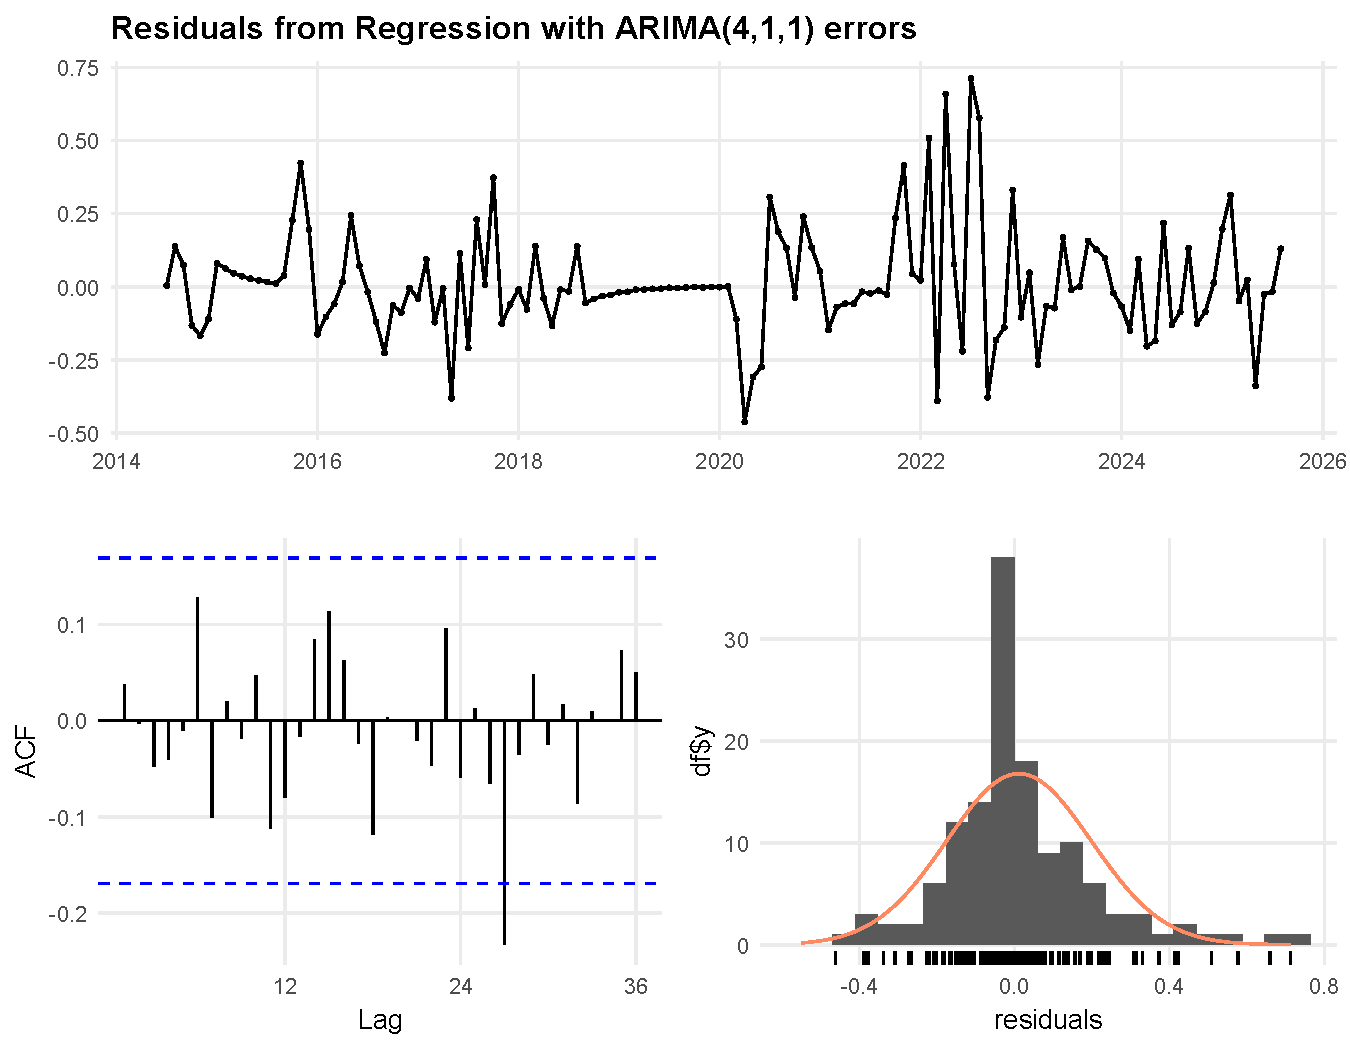
\includegraphics[width=0.95\textwidth]{05_residuos.pdf}
    \caption{Análisis de residuos del modelo ARIMAX(4,1,1) estimado.}
    \label{fig:residuos}
\end{figure}

El diagnóstico del modelo (Figura \ref{fig:residuos}) demuestra la idoneidad del ajuste. El gráfico temporal de los residuos (panel superior) exhibe un comportamiento estable alrededor de cero. La ACF de los residuos (panel inferior izquierdo) muestra que todas las autocorrelaciones caen dentro de las bandas de confianza, indicando ausencia de memoria residual. La prueba formal de Ljung-Box hasta el rezago 24 ($\text{gl} = 19$) arroja $Q = 17.033$ con un $p\text{-valor} = 0.5876 > 0.05$, por lo que no se rechaza la hipótesis nula de independencia, confirmando que el término de error final ($\hat{w}_t$) es, en efecto, Ruido Blanco. Por su parte, el histograma muestra una alta concentración en cero (leptocurtosis, con $p < 0.001$ en Shapiro-Wilk) explicada porque la tasa de interés permanece constante por tramos entre reuniones de la Junta Directiva.

\subsection{Pronóstico y Validación (Out-of-Sample)}
Para evaluar el desempeño predictivo, se reservaron los últimos 12 meses de la muestra (septiembre 2025 a agosto 2026) y se generaron pronósticos fuera de muestra (\textit{ex-post}). La Tabla \ref{tab:metricas} resume los criterios de información AIC y BIC y las métricas de validación RMSE, MAE y MAPE de los tres modelos.

\begin{table}[H]
\centering
\caption{Comparación de criterios de información (AIC y BIC) y métricas de pronóstico en validación ($h=12$).}
\label{tab:metricas}
\vspace{2mm}
\begin{tabular}{llccccc}
\toprule
\textbf{Modelo} & \textbf{Especificación} & \textbf{AIC} & \textbf{BIC} & \textbf{RMSE} & \textbf{MAE} & \textbf{MAPE (\%)} \\
\midrule
ARIMA & $\text{ARIMA}(4,1,1)$ & $-52.78$ & $-35.44$ & $0.994$ & $0.772$ & $6.921$ \\
ARIMA-X (IPI + COVID) & $\text{Reg. ARIMA}(4,1,1)$ (Ec. \ref{eq:ARIMAX_def}) & $-49.28$ & $-26.16$ & $1.009$ & $0.782$ & $7.007$ \\
ARIMA-X rezagos & $\text{Reg. ARIMA}(4,1,1)$ (Ec. \ref{eq:ARIMAX_general}) & $-46.89$ & $-17.99$ & $1.028$ & $0.794$ & $7.100$ \\
\bottomrule
\end{tabular}
\end{table}

\begin{figure}[H]
    \centering
    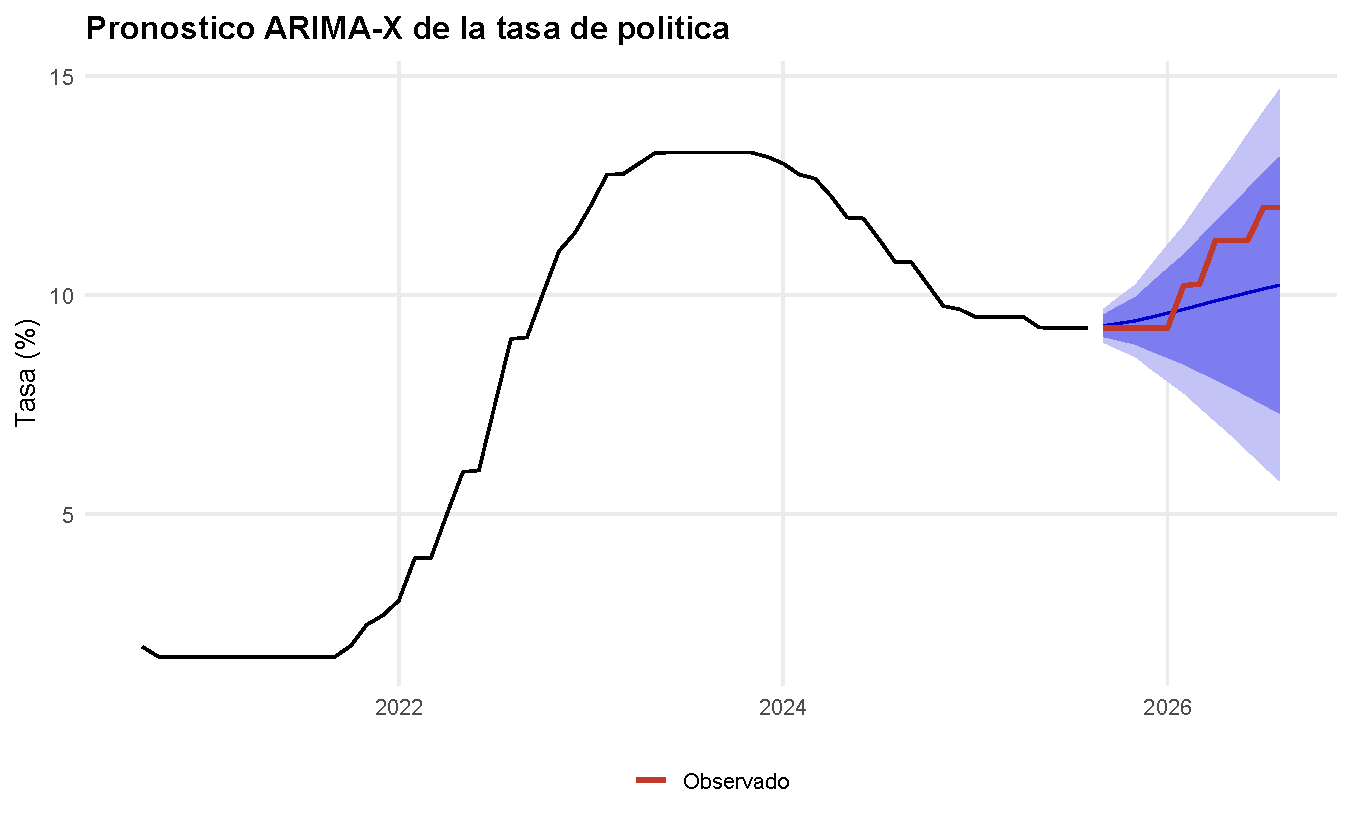
\includegraphics[width=0.85\textwidth]{06_pronostico_arimax.pdf}
    \caption{Pronóstico del modelo ARIMAX con intervalos de confianza del 80\% y 95\%.}
    \label{fig:pronostico}
\end{figure}

La Figura \ref{fig:pronostico} ilustra el pronóstico del modelo ARIMAX. Como es característico en los modelos con un orden de integración $d \ge 1$, la varianza del error de pronóstico crece a medida que aumenta el horizonte $h$, lo que se refleja en el ensanchamiento progresivo de los intervalos de confianza (bandas azules), los cuales logran contener la trayectoria observada de la tasa (línea roja).

\begin{figure}[H]
    \centering
    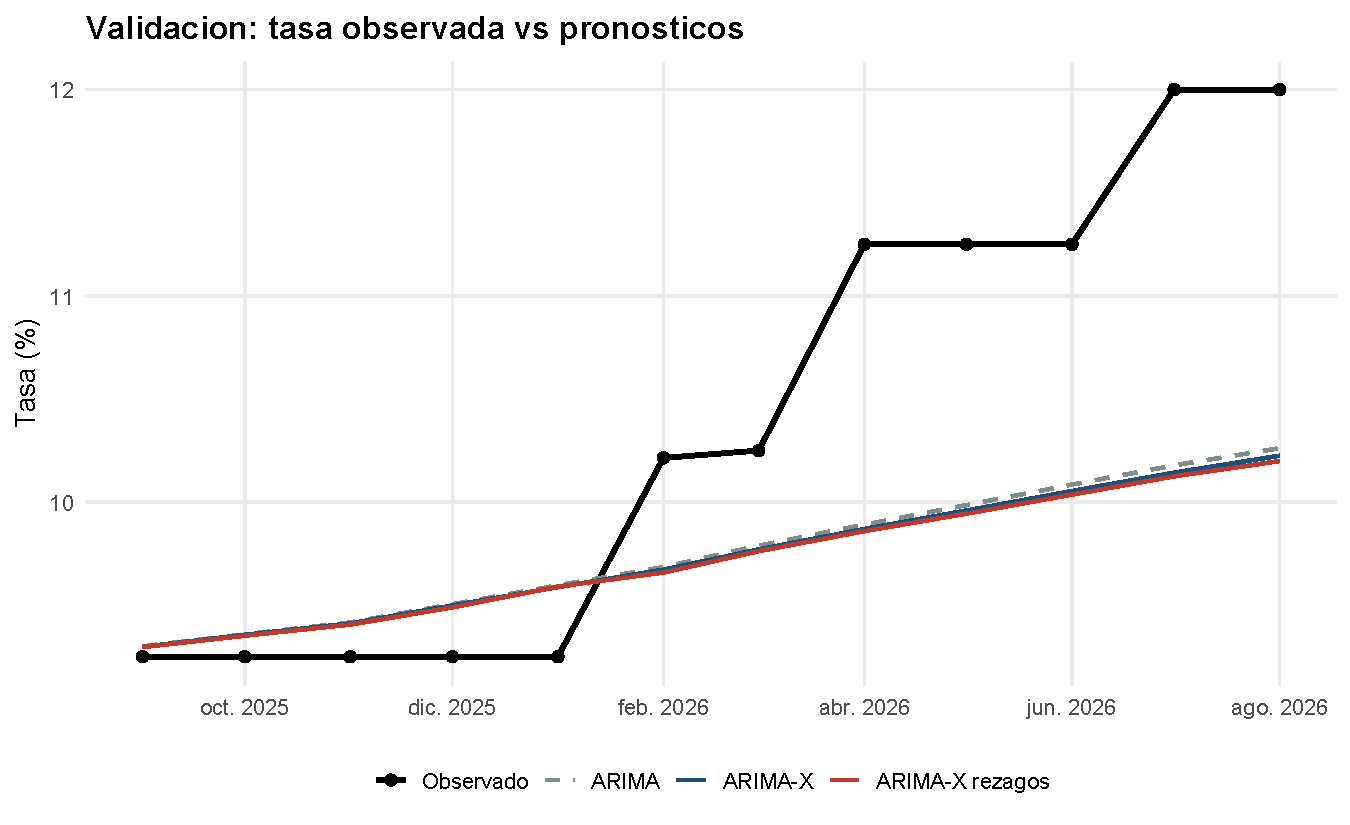
\includegraphics[width=0.85\textwidth]{07_validacion.pdf}
    \caption{Validación fuera de muestra: Valores observados vs. Modelos competitivos.}
    \label{fig:validacion}
\end{figure}

Finalmente, la Figura \ref{fig:validacion} compara la trayectoria real de la Tasa de Intervención (línea negra) frente a los pronósticos de los tres modelos: ARIMA univariado puro, ARIMA-X contemporáneo y ARIMA-X con rezagos. Se evidencia que los tres modelos proyectan acertadamente la tendencia ascendente con errores MAPE cercanos al $7\%$. El hecho de que los modelos que incorporan la información exógena del IPI (líneas azul y roja) proyecten una senda ligeramente más moderada que el ARIMA puro (línea punteada, que obtiene el menor RMSE de $0.994$ y menor AIC de $-52.78$) se explica porque durante 2026 la producción industrial estuvo desacelerada, mientras que el Banco de la República subió la tasa hasta el $12.00\%$ guiado por presiones inflacionarias no incluidas en un modelo bivariado.

%%%%%%%%%%%%%%%%%%%%%%%%%%%%%%%%%
% 9. CONCLUSIONES
% ==========================================
\newpage
\section{Conclusiones}

A partir de los desarrollos teóricos presentados y la evidencia empírica obtenida en la modelación de la Tasa de Intervención del Banco de la República y el Índice de Producción Industrial (IPI) entre enero de 2014 y agosto de 2026, se derivan las siguientes conclusiones fundamentales:

\begin{itemize}
    \item \textbf{Invalidez de MCO en Presencia de Inercia Temporal:} 
    El análisis confirmó que ajustar una regresión lineal clásica mediante Mínimos Cuadrados Ordinarios entre variables macroeconómicas con orden de integración $I(1)$ induce el fenómeno de regresión espuria y genera estimaciones ineficientes. Al no satisfacerse el supuesto de Gauss-Markov de perturbaciones incorrelacionadas ($Var(\boldsymbol{\epsilon}) \neq \sigma^2 \mathbf{I}$), los errores estándar convencionales resultan subestimados, lo que invalida las pruebas de hipótesis $t$ y $F$ al inflar artificialmente la significancia estadística de los coeficientes.

    \item \textbf{Desempeño Estructural de los Modelos ARIMA y ARIMAX:} 
    La formulación con errores $\text{ARIMA}(4,1,1)$ demostró ser indispensable para capturar la fuerte suavización e inercia de la tasa de intervención. Al contrastar las especificaciones mediante los criterios AIC y BIC y las métricas de validación (Tabla \ref{tab:metricas}), se evidenció que los tres modelos logran un desempeño predictivo muy sólido ($\text{MAPE} \approx 7\%$), aunque la persistencia autorregresiva de cuarto orden de la propia tasa domina la predicción de corto plazo y explica por qué el modelo univariado es ligeramente más parsimonioso cuando el sector industrial se desacelera frente a choques inflacionarios.

    \item \textbf{Evidencia de Causalidad Rezagada (El Papel del Pre-blanqueamiento):} 
    La aplicación del procedimiento de pre-blanqueamiento (\textit{prewhitening}) sobre la función de correlación cruzada (Fan, 2009, p. 157) demostró que las decisiones de política monetaria en Colombia no reaccionan de manera instantánea a los cambios de la producción industrial. Los picos estadísticamente significativos en rezagos negativos de la CCF confirman que el sector real actúa como un indicador líder con una ventana de transmisión de entre 3 y 6 meses.

    \item \textbf{Efectividad del Análisis de Intervención y Diagnóstico de Ruido Blanco:} 
    La incorporación de la variable indicadora binaria para el confinamiento por COVID-19 (marzo a octubre de 2020) contribuyó a controlar el choque pandémico. La prueba de Ljung-Box sobre los residuos del modelo estimado ($p\text{-valor} = 0.5876 > 0.05$) y el correlograma sin rezagos significativos ratifican que los errores alcanzaron el comportamiento de Ruido Blanco incorrelacionado, mientras que la leptocurtosis observada en la prueba de Shapiro-Wilk refleja el carácter discreto y escalonado de los ajustes de política monetaria.

    \item \textbf{Dilema Operativo en el Pronóstico Fuera de Muestra:} 
    Si bien el modelo ARIMAX permite evaluar escenarios condicionados a la trayectoria del sector real en la validación \textit{ex-post} (donde se conocen los valores observados del IPI en el periodo de prueba), se subraya una limitación metodológica insoslayable para el pronóstico \textit{ex-ante}: para predecir la tasa de interés en un horizonte $T+h$, es estrictamente obligatorio contar con los pronósticos previos de las covariables exógenas. Conforme el horizonte de predicción $h$ aumenta, la incertidumbre inherente al pronóstico del IPI se transmite hacia la ecuación de la tasa, confirmando que la utilidad operativa del modelo ARIMAX se concentra en el corto y mediano plazo.
\end{itemize}

%%%%%%%%%%%%%%%%%%%%%%%%%%%%%%%%%
\newpage
\section{Referencias Bibliográficas}

\begin{itemize}[label=\textbullet, leftmargin=1.5em, labelwidth=1em, labelsep=0.5em, itemsep=1.2em]
    \item Amézquita Bravo, C. C. (2021). \textit{Evaluación de modelos de series de tiempo para pronosticar la demanda de transporte aéreo a corto y mediano plazo en Colombia} [Tesis de maestría]. Universidad Nacional de Colombia. \url{https://repositorio.unal.edu.co/handle/unal/81124}
    
    \item Box, G. E. P., y Tiao, G. C. (1975). Intervention analysis with applications to economic and environmental problems. \textit{Journal of the American Statistical Association}, \textit{70}(349), 70--79.
    
    \item Chen, C., y Liu, L.-M. (1993). Joint estimation of model parameters and outlier effects in time series. \textit{Journal of the American Statistical Association}, \textit{88}(421), 284--297.
    
    \item DataCamp. (2024). \textit{Exogenous vs. Endogenous Variables: Key Differences and Examples}. \url{https://www.datacamp.com/tutorial/exogenous-vs-endogenous-variable}
    
    \item Fan, J. (2009). The Analysis and Application of ARIMAX Model. En \textit{Proceedings of the Conference on Time Series and Econometric Applications} (pp. 156--159).
    
    \item Hyndman, R. J., y Athanasopoulos, G. (2021). \textit{Forecasting: Principles and Practice} (3.ª ed.). OTexts. \url{https://otexts.com/fpp3/}
    
    \item Ljung, G. M., y Box, G. E. P. (1978). On a measure of lack of fit in time series models. \textit{Biometrika}, \textit{65}(2), 297--303.
    
    \item Ortiz Martín, R. (2022). \textit{Metodología ARIMAX aplicada al análisis de la evolución de datos de suicidios en España} [Trabajo de fin de grado]. Universitat de Barcelona. \url{https://hdl.handle.net/2445/194842}
    
    \item Peña, D. (2005). \textit{Análisis de series temporales}. Alianza Editorial.
    
    \item Shumway, R. H., y Stoffer, D. S. (2017). \textit{Time Series Analysis and Its Applications: With R Examples} (4.ª ed.). Springer.
    
    \item Wei, W. W. S. (2006). \textit{Time Series Analysis: Univariate and Multivariate Methods} (2.ª ed.). Addison-Wesley.
\end{itemize}
 
\end{document}